\documentclass[tikz,border=2pt]{standalone}
\usepackage{amsmath}
\usepackage{pgfplots}
\pgfplotsset{compat=1.18}
\usetikzlibrary{arrows.meta}
\begin{document}
% Convex combinations of x1=(0,0), x2=(4,0), x3=(0,4): p=(1,2) has weights (1/4,1/4,1/2) and equals
% (1/2)y3+(1/2)x3 with y3=(2,0) on the opposite side; q=(3,2) has weights (-1/4,3/4,1/2) and lies outside.
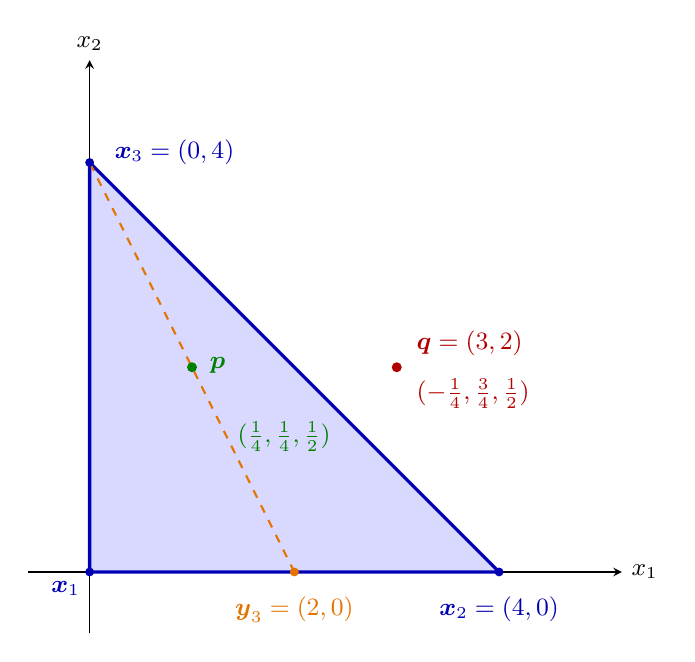
\begin{tikzpicture}[font=\small, >={Latex[length=2mm]}]
  \begin{axis}[
    axis lines=middle, xmin=-0.6, xmax=5.2, ymin=-0.6, ymax=5,
    xtick=\empty, ytick=\empty,
    xlabel={$x_1$}, ylabel={$x_2$},
    xlabel style={anchor=west}, ylabel style={anchor=south},
    x=1.3cm, y=1.3cm, clip=false
    ]
    \fill[blue!15] (axis cs:0,0) -- (axis cs:4,0) -- (axis cs:0,4) -- cycle;
    \draw[blue!70!black, very thick] (axis cs:0,0) -- (axis cs:4,0) -- (axis cs:0,4) -- cycle;
    \draw[orange!90!black, thick, dashed] (axis cs:2,0) -- (axis cs:0,4);
    \fill[blue!70!black] (axis cs:0,0) circle (1.6pt);
    \fill[blue!70!black] (axis cs:4,0) circle (1.6pt);
    \fill[blue!70!black] (axis cs:0,4) circle (1.6pt);
    \node[blue!70!black, anchor=north east] at (axis cs:0,0) {$\boldsymbol{x}_1$};
    \node[blue!70!black, anchor=north] at (axis cs:4,-0.15) {$\boldsymbol{x}_2=(4,0)$};
    \node[blue!70!black, anchor=west] at (axis cs:0.15,4.1) {$\boldsymbol{x}_3=(0,4)$};
    \fill[orange!90!black] (axis cs:2,0) circle (1.6pt);
    \node[orange!90!black, anchor=north] at (axis cs:2,-0.15) {$\boldsymbol{y}_3=(2,0)$};
    \fill[green!50!black] (axis cs:1,2) circle (1.8pt);
    \node[green!50!black, anchor=west] at (axis cs:1.08,2.02) {$\boldsymbol{p}$};
    \node[green!50!black, anchor=north west] at (axis cs:1.35,1.56) {$(\tfrac{1}{4},\tfrac{1}{4},\tfrac{1}{2})$};
    \fill[red!70!black] (axis cs:3,2) circle (1.8pt);
    \node[red!70!black, anchor=south west] at (axis cs:3.1,2.02) {$\boldsymbol{q}=(3,2)$};
    \node[red!70!black, anchor=north west] at (axis cs:3.1,1.98) {$(-\tfrac{1}{4},\tfrac{3}{4},\tfrac{1}{2})$};
  \end{axis}
\end{tikzpicture}
\end{document}
